\begin{appendix}
\section{Flow charts}
\label{app:charts}
\begin{figure}[h!]
\begin{center}
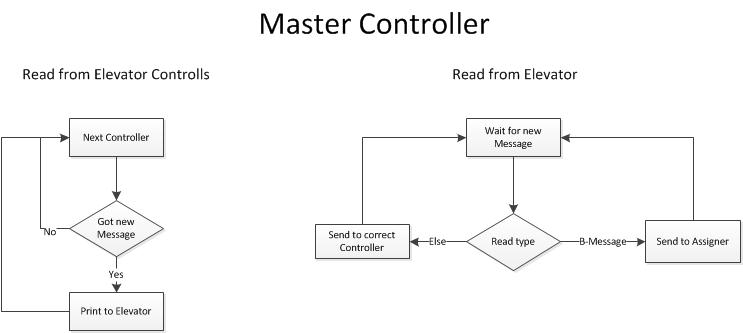
\includegraphics[scale=0.8]{FlowChart/MasterC.jpg}
\caption{Flowchart for MasterController.}
\label{chart:master}
\end{center}
\end{figure}

\begin{figure}[h!]
\begin{center}
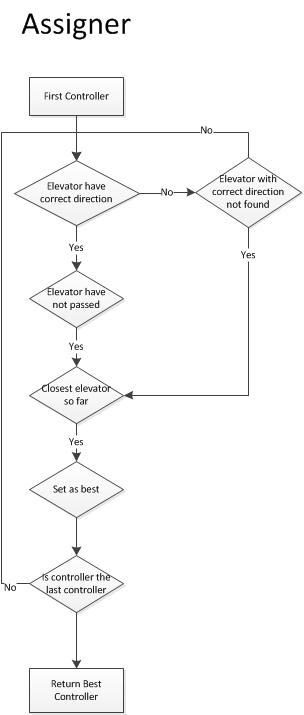
\includegraphics{FlowChart/Assigner.jpg}
\caption{Flowchart for Assigner.}
\label{chart:assigner}
\end{center}
\end{figure}

\begin{figure}[h!]
\begin{center}
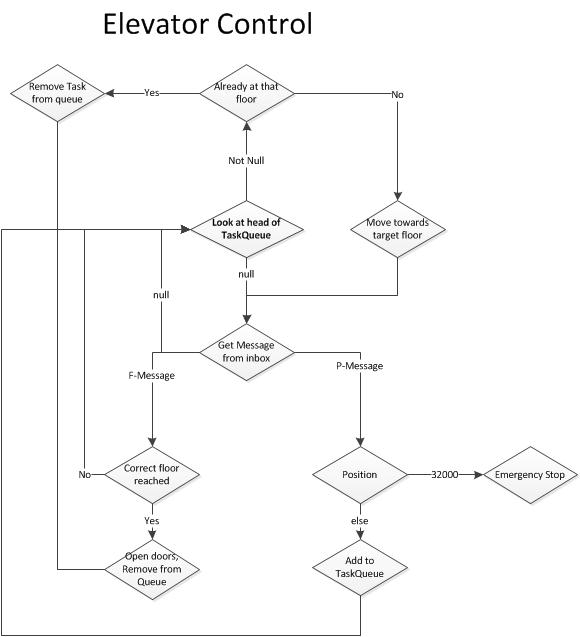
\includegraphics{FlowChart/ElevatorControll.jpg}
\caption{Flowchart for ElevatorController.}
\label{chart:controller}
\end{center}
\end{figure}

\begin{comment}
\section{README}
\label{code:readme}
\lstinputlisting{../src/controller/README}

\section{Makefile}
\label{code:makefile}
\lstinputlisting{../src/controller/Makefile}

\end{comment}
\cleardoublepage
\section{MasterController.java}
\label{code:master}
\lstinputlisting{../src/controller/MasterController.java}

\section{ElevatorController.java}
\label{code:controller}
\lstinputlisting{../src/controller/ElevatorController.java}

\section{Message.java}
\label{code:message}
\lstinputlisting{../src/controller/Message.java}
\end{appendix}
